\documentclass{article}
\usepackage[utf8]{inputenc}
\usepackage{geometry}[margins = 1in]
\usepackage{graphicx}
\usepackage{hyperref}
\usepackage{eufrak}
\usepackage{fullpage}
\usepackage{amsmath}
\usepackage{listings}
\usepackage[makeroom]{cancel}
\usepackage{color}
\usepackage{amssymb}
\usepackage{float}
\floatplacement{figure}{H}
\setkeys{Gin}{width=0.75\linewidth}

\hypersetup{
    colorlinks=true, %set true if you want colored links
    linktoc=all,     %set to all if you want both sections and subsections linked
    linkcolor=blue,  %choose some color if you want links to stand out
}


\newcommand{\unit}[1]{{\,\rm #1}}
\newcommand{\be}{\begin{equation}}
\newcommand{\ee}{\end{equation}}
\newcommand{\Mpc}{\unit{Mpc}}
\newcommand{\Gpc}{\unit{Gpc}}
\newcommand{\Gyr}{\unit{Gyr}}
\newcommand{\s}{\unit{s}}
\newcommand{\km}{\unit{km}}
\newcommand{\yr}{\unit{yr}}
\newcommand{\g}{\unit{g}}
\newcommand{\cm}{\unit{cm}}
\newcommand{\frw}{\mathrm{d}s^2 = c^2 \mathrm{d}t^2 - a^2\left(t\right) \left[\frac{\mathrm{d}r^2}{1-kr^2} + r^2 \left(\mathrm{d}\theta^2 + \sin^2\theta \mathrm{d}\phi^2\right) \right]}


%%%%%
\def\:{\ddot }
\def\.{\dot }
\def\^{\hat }
\def\_{\bar }
\def\~{\tilde }
\def\hf{\frac12}
\def\imply{\Rightarrow}
\def\inv#1{\frac{1}{ #1}}
\def\ddt{\frac{d}{dt}}
\def\aa{\frac{\dot a }{ a}}
\def\adda{\frac{\ddot a}{ a}}
\def\thnot{\theta_0}
\def\etot{\Omega_0}
\def\econs{\Omega_{0,\Lambda}}
\def\emat{\Omega_{0,M}}
\def\econs{\Omega_{0,\Lambda}}
\def\p{^\prime}
\def\iff{\Leftrightarrow}
\def\xv{{\vec x}}
\def\pv{{\vec p}}
\def\vv{{\vec v}}
\def\ppt{\frac{\partial}{\partial t}}
\def\ddt{\frac{d}{dt}}
\def\epot{\frac{8\pi}{ 3}}
\def\attw{a^{3+3w}}
\def\athow{a^{-\frac{3}{2}(1+w)}}
\def\atow{a^{-3(1+w)}}
\def\atowi{a^{-3(1+w_i)}}
\def\hf{\frac12}
\def\imply{\Rightarrow}
\def\thnot{\theta_0}
\def\etot{\Omega_0}
\def\econs{\Omega_{0,\Lambda}}
\def\emat{\Omega_{0,M}}
\def\econs{\Omega_{0,\Lambda}}
\def\p{^\prime}
\def\iff{\Leftrightarrow}
\def\xv{{\vec x}}\def\pv{{\vec p}}
\def\vv{{\vec v}}
\def\ddt{{\frac{d}{dt}}}
\def\atow{a^{-3(1+w)}}
\def\atowi{a^{-3(1+w_i)}}
\def\attw{a^{3+3w}}
\def\cc{Cosmological constant}
\def\jumble{\frac{\Omega _0}{ \attw} + \frac{1 - \Omega _0}{ a^2}}
\def\jimble{\sqrt{\Omega _{0,m}(1+z)^3+\Omega _{0,\Lambda}+(1-\Omega _{0,m}-\Omega _{0,\Lambda})(1+z)^2}}
\def\paap{\left(\aa\right)}
\def\rcr{{\rho_{crit}}}




\title{Extragalactic Astrophysics and Comsology}
\author{Jacob Pilawa}
\date{Spring 2021}

\begin{document}

\maketitle
\tableofcontents
\newpage

\section{The Smooth Universe}
\subsection{The Cosmological Principle; The Hubble Parameter; Scale Factor}

\subsubsection{The Cosmological Principle}

We begin with \textbf{The cosmological Principle}. It sounds simple, but incredibly well supported. It says that \textbf{the Universe (spatially) is homogeneous and isotropic on very large spatial scales}. Observationally, this is around $100 \Mpc$ scales. Homogeneous means constant density (non-realistically, this is mass density; relativistic ally, this is energy density). Isotropic means the same in all directions. 

\textit{Note}: Isotropy about $2$ points (or more) implies homogeneity. Isotropy about $1$ point is not enough. Here is a quick illustration of that: 

\begin{figure}
    \centering
    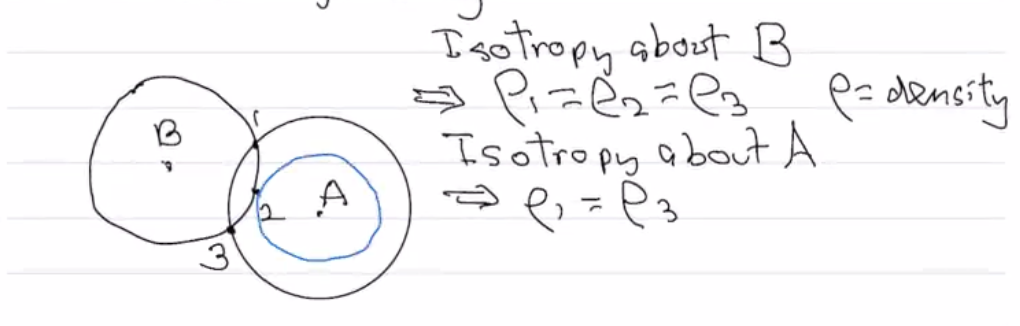
\includegraphics{isotropy.png}
    \caption{Istropy aobut 2 points.}
    \label{fig:isotropy}
\end{figure}

We can consider another example. A homogeneous universe can anisotropic. Consider a homogeneous Universe that is expanding in different directions in a non-uniform way. This leads to different $H_0(x,y,z)$. 

The reason we spend some time on the Cosmological Principle is the \textbf{Friedmann-Robertson-Walker metric}, which we will come to later on.

\subsubsection{Hubble Parameter}

Let's now talk about the \textbf{Hubble parameter}, which is not a constant! It, in fact, changes in time. An empirical linear relationship between the recession speed $v$ and distance $r$ can be seen, called the \textbf{Hubble's Law}:

\begin{equation}
v = H r
\end{equation}

Note that $H_0$ has units of $1/$time. One convention to note is that:

\begin{equation}
H = 100 \underbrace{h}_\text{to hide our ignorance} \frac{\km}{\s \Mpc}
\end{equation}

One useful number to know is $H \approx \frac{h}{10^{10} \yr}$.

Sometimes, when we write $H_0$, we mean the ``present-day'' value ($z = 0$). This is how we will use it now.

\subsubsection{Scale Factor}

We need a language to describe the expansion of the Universe. We will use $a(t)$, which describes the expansion (or contraction) of the Universe. It also relates two different coordinate systems: physical coordinates $\vec{r}$ to comoving coordinates $\vec{x}$. The relation:

\begin{equation}
    \vec{r} = a(t) \vec{x}
\end{equation}

We typically use comoving coordinates in calculations in Cosmology. We can think of $\vec{x}$ as the notches on a stretching ruler. Now consider:

\begin{equation}
    \frac{d}{dt}\vec{r} = \vec{v} = \dot{a} \vec{x} a \vec{\dot{x}}
\end{equation}

\begin{equation}
    \frac{d}{dt}\vec{r} = \vec{v} = \dot{a} \vec{x} a \vec{\dot{x}} = \underbrace{\frac{\dot{a}}{a} \vec{r}}_\text{Hubble} + \underbrace{a \vec{\dot{x}}}_\text{motion relative to expansion (``peculiar velocity'')}
\end{equation}

\begin{equation}
    \boxed{H(t) = \frac{\dot{a}(t)}{a(t)}}
\end{equation}

The name of the game for measuring $H$ is to go far enough that the first term dominates. Otherwise, locally, the second term dominates since peculiar velocities are of order $100$s of $\km/\s$. 

One other convention we need to establish:

\begin{equation}
    a(t_0) = 1 \rightarrow \text{comoving} = \text{today}
\end{equation}

\subsection{The Friedmann Equation; The Equation of State; Radiation, Matter, and Dark Energy}

\subsubsection{The Friedmann Equation}

Below, we will use and derive these, but I am putting the equations at the top for convenience. 

\begin{equation}
    \boxed{\left(\frac{\dot{a}}{a}\right)^2 = \frac{8\pi}{3} G \rho - \frac{kc^2}{a^2}}
\end{equation}

\begin{equation}
    \boxed{\dot{\rho} = -3 \frac{\dot{a}}{a} \left(P + \rho\right)}
\end{equation}

\begin{equation}
    \boxed{\frac{\ddot{a}}{a} = - \frac{4\pi G}{3}\left(\rho +  3P\right)}
\end{equation}

Let's motivate the origin with quasi-Newtonian physics. We can derive it from General Relativity, but that's overkill.

If we assume isotropy, we only need to worry aobu the radial coordinate $r$, not $\theta$ or $\phi$. Homogeneity tells us that $\rho = \text{constant}$ spatially, but \textit{can} depend on time. We will model the Universe as an expanding, homogeneous medium that is adiabatically ($\Delta s =0$) expanding. If it were not adiabatically expanding, we would have heat flow and thus no isotropy. 

With these conditions, let's examine the motion of a thin, expanding, spherical shell of radius $a$. This depends \textbf{only} on the enclosed mass within $a$\footnote{see Birkhoff's Theorem for General Relativity proof}:


\begin{equation}
    M(<a) = \frac{4}{3}\pi a^3 \rho
\end{equation}

Let's consider the energy:


\begin{equation}
    E = \frac12 \dot{a}^2 - \frac{GM}{a}
\end{equation}


\begin{equation}
E = \frac12 \dot{a}^2 - \frac43 \pi G \rho a^2
\end{equation}

Let's re-write $E$ a bit: $k c^2 \equiv -2E$. Note that $k \propto 1/\text{length}^2$. There are three possibilities for $kc^2$:

\begin{itemize}
    \item $>0$, $E<0$, bound
    \item $=0$, $E=0$, critical
    \item $<0$, $E>0$, unbound
\end{itemize}

Let's now evoke the First Law of Thermodynamics ($\Delta S = 0$):

\begin{equation}
   \underbrace{\mathrm{d}U}_\text{internal energy} = -P \mathrm{d}V 
\end{equation}

We now equation the internal energy to the rest-mass energy:

\begin{equation}
    \mathrm{d}\left(\rho c^2 a^3\right) = -P \mathrm{d}\left(a^3\right)
\end{equation}

We will now set $c = 1$ and take a time derivative:

\begin{equation}
    \dot{\rho} a^3 + 3 \rho a^2 \dot{a} = -3P a^2 \dot{a}
\end{equation}

\begin{equation}
    \dot{\rho} -3\frac{\dot{a}}{a}\left(P + \rho\right)
\end{equation}

Using this result and the energy equation from above

\begin{equation}
    \left(\frac{\dot{a}}{a}\right)^2 = \frac{8\pi}{3}G \rho - \frac{k (c)^2}{a^2}
\end{equation}

to get a new equation. If you stare at it hard enough and have divine intervention, take a derivative of the second equation and multiply by $a^2$. Doing so, you get:

\begin{equation}
    2 \dot{a} \ddot{a} = \frac{8\pi}{3}G\frac{d}{dt}(\rho a^2) = \frac{8\pi}{3}Ga^2\left(\dot{\rho} + 2\frac{\dot{a}{a}}\rho\right)
\end{equation}

Simplifying with the other above equation, we get:

\begin{equation}
    2\dot{a}\ddot{a} = -\frac{8\pi}{3}Ga^2 \left(\frac{\dot{a}}{a}\rho + 3\frac{\dot{a}}{a}P\right)
\end{equation}

Simplifying:

\begin{equation}
    \frac{\ddot{a}}{\dot{a}} = -\frac{4\pi}{3}G \left(\rho + 3P\right)
\end{equation}

Note that this is not independent from the other equations; rather it is massaged. Let's compare this to $1$-D Newtonian forces:

\begin{equation}
    \ddot{x} = -\frac{GM}{x^2} = -\frac{4}{3}\pi G \rho x
\end{equation}

\begin{equation}
    \frac{\ddot{x}}{x} = -\frac{4}{3}\pi G \rho 
\end{equation}

Had we done strictly Newtonian physics, we would have never gotten the $+3P$ term. The way to interpret this: we can think of $\rho$ to have an extended meaning: $\rho_{eff} = \rho + 3P$. 

The Grand Summary so far: two equations of motion for $a(t)$: 

\begin{equation}
    \frac{\ddot{a}}{\dot{a}} = -\frac{4\pi}{3}G \left(\rho + 3P\right)
\end{equation}

\begin{equation}
    \dot{\rho}= -3\frac{\dot{a}}{a}\left(P + \rho\right)
\end{equation}

Note this second equation tells us the acceleration! Very importantly, we have a minus sign. If $\rho$ and $P$ are positive, the Universe is \textbf{decelerating}! Conversely, if you have a \textit{bizarre} $P$ and could reverse the parenthetical term, we can have accelerated expansion! 


Right now, we have three unknowns ($P, \rho, a$). How do we get that last piece -- the equation of state ($P \iff \rho$ dependence)?

\subsubsection{Equation of State}

We choose to write:

\begin{equation}
    P = w\rho (c^2)
\end{equation}

We are in units where $c = 1$, but I threw it in for reference. Note -- this means that pressure is the same thing as energy density! Think of the units. 

With that definition of $P$, we can re-write the second boxed equation from above:

\begin{equation}
    \dot{\rho} -3\frac{\dot{a}}{a}\left(1+w\right)\rho
\end{equation}

\begin{equation}
    \frac{\dot{\rho}}{\rho} = -3 (1+w) \frac{\dot{a}}{a} \rightarrow \rho \propto a ^{-3(1+w)}
\end{equation}

\begin{equation}
    \boxed{\rho \propto a^{-3\left(1+w\right)}}
\end{equation}

\textbf{assuming that} $\dot{w} =0$ \textbf{which might not be true}!

\subsubsection{Matter, Radiation, and Dark Energy}

Let's look at a few special cases of the equation of state:

\begin{itemize}
    \item Matter: Non-relativistic, pressure-less particles like cold dark matter. In this case, $w = 0, P = 0 \rightarrow \boxed{\rho \propto a^{-3}}$. This makes sense because it is units of $1/\text{volume}$.
    \item Radiation: Relativistic particles, photons and neutrinos. In this case, $w = 1/3, P = \frac13 \rho \rightarrow \boxed{\rho \propto a^{-4}}$. This makes sense because it is units of $\left(1/\text{volume}\right)\left(1/\text{length}\right) $ where the extra factor is from redshifting energy.
    \item The Cosmological Constant: In this case, $w = -1, P=-\rho \rightarrow \rho = \text{constant}$.
    \item Dark Energy: More general term, where $w < -\frac13$ to make $\ddot{a} >0$.
\end{itemize}

\begin{figure}
    \centering
    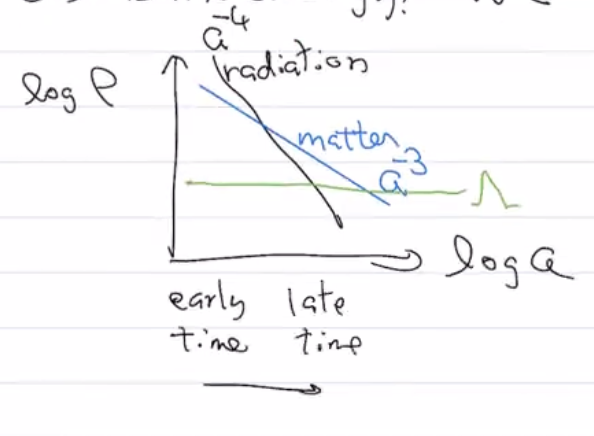
\includegraphics{density.png}
    \caption{Sketch of density over cosmic time. }
    \label{fig:density}
\end{figure}

\subsection{The Density Parameter; Open, flat, closed models; Redshift}

Let's first define $\Omega$ in terms of the \textbf{critical density} $\rho_c$. This is defined to be the density needed to make the Universe flat. Recall the Friedmann Equation:

\begin{equation}
    \left(\frac{\dot a}{a}\right)^2 = \frac{8\pi}{3}G\rho - \frac{k}{a^2}
\end{equation}

First, set $k = 0 \iff E = 0$, then solve for $\rho$:

\be
    \boxed{\rho_c = \frac{3H^2}{8\pi G}}
\ee

This critical density can be interpreted as well as the mean density of a flat Universe ($k=0$). Importantly, $\rho_c$ is a function of $H$, which itself is a function of time. Setting $H = H_0$, we can get Today's value of $\rho_c$:

\be
    \rho_{c,0} = \frac{3H_0^2}{8\pi G} = 2.78 \times 10^{11} h^2 \frac{M_\odot}{\Mpc^3} = 1.88 \times 10^{-29} h^2 \frac{\g}{\cm^3}
\ee

This is about $10^{-5} h^2 m_{proton} \cm^{-3}$. Here are a few other useful numbers to carry around as well:

\be
    \rho_{thumb} \sim 1 \frac{\g}{\cm^3}
\ee

\be
    \rho_{ISM} \sim 1 \frac{m_p}{\cm^3}
\ee

\be
    \rho_{Universe} \sim 1 \rho_c
\ee

Now with these definitions, we have the \textbf{density paramater}:

\be
\Omega(t) \equiv \frac{\rho(t)}{\rho_c(t)} = \frac{8\pi G \rho(t)}{3H^2(t)}
\ee

There are three obvious possibilities:

\begin{itemize}
    \item $\Omega <1 \rightarrow$ Open Universe ($k<0$)
    \item $\Omega = 1\rightarrow$ Flat Universe ($k=0$)
    \item $\Omega >1 \rightarrow$ Closed Universe ($k>0$)
\end{itemize}

There are a few things to note. When we have \textit{mutliple components}, we have:

\be
\Omega(t) = \frac{\sum_{i} \rho_i}{\rho_c}
\ee

where $i$ is often representing radiation, matter, $\Lambda$, baryonic component of matter, dark matter, neutrinos, etc. Another thing we want to stress is that $\rho$, $\rho_c$, $\Omega$ \textbf{all depend on time}. Note that if $\rho > \rho_c$, it will STAY that way. The same goes for $\Omega$, and for other values. For example, these parameters will stay $>, <,$ or $=$ 1. 

\subsubsection{Redshift}

Observationally, we have

\be
1+z \equiv \frac{\lambda_{obs}}{\lambda_{rest}} = \frac{a(t_0)}{a(t)} = \frac{1}{a(t)}
\ee

\be
\boxed{\frac{1}{a(t)} = 1+z}
\ee

\subsection{Time Evolution of Paramaters: Hubble, Density, Scale Factor}

\subsubsection{Hubble Parameter}

Worked out in Problem Set 1, but here is the solution:

\be
H^2(a) = H_0^2 \left(\frac{\Omega_0}{a^{3+3w}} + \frac{1-\Omega_0}{a^2}\right)
\ee

For multiple components (the common ones):

\be
H^2(a) = H_0^2 \left(\frac{\Omega_{0,m}}{a^{3}} + \Omega_{0,\Lambda} + \frac{\Omega_{0,r}}{a^{4}}+ ... + \frac{1-\Omega_{0,m}-\Omega_{0,\Lambda}-\Omega_{0,r}}{a^2}\right)
\ee

\subsubsection{Density Parameter}

First, recall the critical density:

\be
\rho_c = \frac{3 H^2}{8\pi G} \rightarrow H^2 \Omega = \frac{8\pi}{3}G\rho
\ee

We can also look at the Friedmann equation:

\begin{equation}
    \left(\frac{\dot a}{a}\right)^2 = \frac{8\pi}{3}G\rho - \frac{k}{a^2}
\end{equation}

We can replace the first term on the right hand side and set $a=1$:

\be
k = H_0^2 \left(\Omega_0-1\right)
\ee

All of these together, we get:

\be
H^2 = H^2 \Omega - \frac{H_0^2 \left(\Omega_0-1\right)}{a^2}
\ee

Rearrange:

\be
1 - \Omega(a) = \frac{H_0^2}{H^2a^2}\left(1-\Omega_0\right)
\ee

We can use the time evolution of the Hubble Parameter to replace the $H$ terms, leaving:

\be
\boxed{1-\Omega(a) = \frac{1-\Omega_0}{\frac{\Omega_0}{a^{1+3w}} + 1-\Omega_0   }}
\ee

To be more explicit, let's write out the multi-component again:

\be
1 - \Omega(a) = \frac{1 - \Omega_0}{1 - \Omega_0 + \left(\Omega_{m,0}a^{-1} + \Omega_{0,\Lambda}a^{2} + \Omega_{r,0}a^{-2}\right)}
\ee

where $\Omega_0 = \sum_i \Omega_{0,i}$. Note that the above equation essentially FORCES $\Omega(a) \sim 1$. This foreshadows the Flatness Problem.

\subsubsection{Scale Factor (Flat Case)}

This is essentially solving the Friedmann Equation for $a(t)$ for specific models (can, in general, be integrated). The most basic model is the Einstein-de Sitter model: a model that is flat $k = 0 \rightarrow \Omega =1$:

\be
\left(\frac{\dot a}{a}\right)^2 = \frac{8\pi}{3}G\rho
\ee

We have also see that $\rho \propto a^{-3(1+w)}$. Therefore:

\be
\mathrm{d} a a^{\frac32 (1+w)-1} \propto \mathrm{d}t
\ee

\be
\boxed{a(t) \propto t^{\frac{2}{3(1+w)}}}
\ee

Recall for the Einstein-de Sitter model ($k=0, \Omega=0$), we found:

\be
a \propto t^{\frac{2}{3(1+w)}}
\ee

This is very useful since it works for each epoch (matter dominated, radiation dominated, dark energy dominated, etc;, but not in the transitions):

\textbf{Matter Dominated Era} ($w=0, P\approx0$)

\begin{equation}
    \boxed{a_{m}\propto t^{\frac23}}
\end{equation}

\textbf{Radiation Dominated Era} ($w=\frac13, P=\frac13 \rho$)

\begin{equation}
    \boxed{a_{r}\propto t^{\frac12}}
\end{equation}

$\Lambda$ \textbf{Dominated Era} ($w=-1$ (for example), $P=-\rho$)

\begin{equation}
    a_{r}\propto t^{\infty} \rightarrow \text{ Wrong! }
\end{equation}

This breaks down because $H$ is a constant in this case! So here:

\be
    a \propto e^{Ht}
\ee

Isn't this reminiscent of inflation? That's because it is! It wasn't the Cosmological Constant but rather a scalar field called the inflaton.  


\subsubsection{Scale Factor (Open Case)}

Let's consider $k<0$ and $\Omega <1$. Additionally, we assume $\Lambda =0$ and that we are matter-dominated. 

Start with the Friedmann Equation:

\be
\frac{\dot a^2}{a^2} = \frac{8\pi}{3}G\rho - \frac{k}{a^2} > 0 \text{ always}
\ee

Immediately, we see that expansion will never stop! The right hand side is always positive, and therefore $\dot a$ is never equal to $0$. Now, recall the equation for $H(a)$ and the fact that $H = \dot{a}/a$:

\be
\dot{a}^2 = H_0^2 \left(\frac{\Omega_0}{a^{1+3w}} + 1 - \Omega_0\right)
\ee

We now solve for $a(t)$ for this Universe:

\be
\int_0^{a_f} \frac{\mathrm{d}a}{\sqrt{\frac{\Omega_0}{a} + 1 - \Omega_0}} = \int_0^{t_f} H_0 \mathrm{d}t
\ee

The right hand side is easy. The left hand side? Let's start with completing the squares to get rid of the $\frac{1}{a}$, so let's set that up.

\be
\int_0^{a_f} \frac{a \mathrm{d}a}{\left(1-\Omega_0\right)\sqrt{a^2 + \frac{\Omega_0}{1-\Omega_0}a }}
\ee

Now we can actually complete the square in the denominator. Define $2\alpha\equiv \frac{\Omega_0}{1-\Omega_0}$:

\be
\int_0^{a_f} \frac{a\mathrm{d}a}{\sqrt{1-\Omega_0} \sqrt{\left(a + \alpha\right)^2 - \alpha^2}}
\ee

We will now shift variables: $a\prime \rightarrow a + \alpha$:

\be
\int_\alpha^{a_f + \alpha} \frac{\left(a-\alpha\right)\mathrm{d}a}{\sqrt{1-\Omega_0} \sqrt{a^2 - \alpha^2}}
\ee

We can now do trigonometric substitution. Let $a\equiv \alpha \cosh \theta$. This gives $\mathrm{d}a = \alpha \sinh\theta \mathrm{d}\theta$. Lastly, $\sqrt{a^2\alpha^2} = \alpha\sinh\theta$. Properly adjusting limits, we get the expression:

\be
\boxed{a(\theta) = \frac{\Omega_0}{2\left(1-\Omega_0\right)}\left(\cosh\theta-1\right)}
\ee

\be
\int_{0}^{\theta_f} \frac{\alpha^2\left(\cosh\theta-1\right)\sinh\theta}{\sqrt{1-\Omega_0} \alpha \sinh\theta} \mathrm{d}\theta
\ee

\be
\frac{\alpha}{\sqrt{1-\Omega_0}}\left(\sinh\theta - \theta\right)\rvert_0^{\theta_f}
\ee

\be
H_0 t_f = \frac{\Omega_0}{2\left(1-\Omega_0\right)^{3/2}} \left(\sinh\theta_f -\theta_f\right)
\ee

This gives:

\be
\boxed{t(\theta) = \frac{\Omega_0}{2H_0\left(1-\Omega_0\right)^{3/2}}\left(\sinh\theta - \theta\right)}
\ee

We can then use $\theta$ as some parameter, trace out $a$ and $t$, and then find $a(t)$!

\subsubsection{Scale Factor (Closed Case)}

You can repeat the derivation above for the matter-dominated, closed case of $k >0$, $\Omega > 1$. Here, there \textit{will} be a maximum of $a$ and the dynamics are different $\theta \rightarrow i \theta$):

\be
\boxed{t(\theta) = \frac{\Omega_0}{2H_0\left(\Omega_0-1\right)^{3/2}}\left(\theta-\sin\theta\right)}
\ee

\be
\boxed{a(\theta) = \frac{\Omega_0}{2\left(\Omega_0-1\right)}\left(1-\cos\theta\right)}
\ee

\subsubsection{Deceleration Parameter}

Let's define this -- it was used historically since we now know the Universe is \textit{accelerating}. This is a dimensionless parameter:

\be
q \equiv -\frac{\ddot{a}a}{\dot{a}^2} \rightarrow q = - \frac{1}{H^2} \frac{\ddot{a}}{a}
\ee

Recall one of the other results we had this semester:

\be
\frac{\ddot{a}}{a} = -\frac{4\pi}{3}G\left(\rho+3P\right)
\ee

and

\be
\rho_c = \frac{3H^2}{8\pi G} \rightarrow H^2 \Omega = \frac{8\pi}{3}G\rho
\ee

Putting this together with $q$:

\be
\frac{\ddot{a}}{a} = -\frac{4\pi}{3}G\rho \left(1+3w\right) = -\frac{H^2 \Omega}{2}\left(1+3w\right)
\ee

This makes:

\be
q = \frac{\Omega}{2}\left(1+3w\right)
\ee

For multiple components:

\be
\boxed{q = \sum_i \frac{\Omega_i}{2}\left(1+3w_i\right)}
\ee

\be
q = \frac{\Omega_m}{2} + \underbrace{\frac{1+3w}{2}\Omega_w}_\text{Dark Energy} + \Omega_r + ...
\ee

For a matter-dominated Universe and $\Omega_\Lambda \neq 0$:

\be
\boxed{q = \frac{\Omega_m}{2} - \Omega_\Lambda}
\ee

\textbf{The minus sign there is enormously important!}

One thing to note: supernovae are sensitive to $q$, whereas CMB measurements are sensitive to the addition of $\Omega_m$ and $\Omega_\Lambda$, so in some sense, these are orthogonal instead of parallel. 

\subsection{Robertson-Walker Metric}

This is where you would start in General Relativity. 

Let's set up the background. Recall Lorentz transformations in Special Relativity. There are two inertial observers, $(x,y,z,t)$ and $(x',y',z',t')$ with relative velocity $\vec{v}=v\hat{x}$:

\be
x' = \gamma(x-vt)
\ee

\be
y' = y
\ee

\be
z' = z
\ee

\be
t' = \gamma\left(t-\frac{vx}{c^2}\right)
\ee

We also talked about the Lorentz invariant interval:

\be
\mathrm{d}s^2 = c^2 \mathrm{d}t^2 - \left(\mathrm{d}x^2 + \mathrm{d}y^2 + \mathrm{d}z^2\right) = \mathrm{d}s'^2
\ee

Recall that the propagation of light follows the ``null geodesic'': $\mathrm{d}s^2 = 0$:

\be
\mathrm{d}r = c\mathrm{d}t
\ee

We will quote the RW Metric here, and explore it next time. In short, Robertson and Walker showed that, for a \textbf{homogeneous and isotropic space, the most general metric is} (see Weinberg for a full proof):

\be
\mathrm{d}s^2 = c^2 \mathrm{d}t^2 - a^2\left(t\right) \left[\frac{\mathrm{d}r^2}{1-kr^2} + r^2 \left(\mathrm{d}\theta^2 + \sin^2\theta \mathrm{d}\phi^2\right) \right]
\ee

We are defining the coordinates as:

\begin{figure}
    \centering
    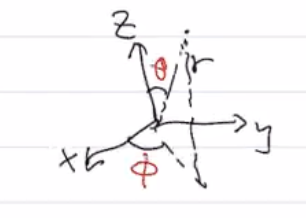
\includegraphics[width=0.75\textwidth]{coordinates.png}
    \caption{Spherical coordinate convention. }
    \label{fig:coords}
\end{figure}

An immediate and obvious consequence is when $k=0$, where we recover the Minkowski metric for flat space. 
Let's consider the more interesting cases of open ($k<0$) and closed ($k>0$). Immediately, we have a coordinate singularity at $r = \frac{1}{\sqrt{k}}$. Recall that $k = \frac{H_0^2}{c^2} \left(\Omega_0-1\right)$. We can thus define the \textbf{radius of curvature}:

\be
R_0 \equiv \frac{1}{\sqrt{k}} = \frac{c}{H_0} \left(\frac{1}{\sqrt{\Omega_0-1}}\right)
\ee

Let's step back a second and look at the form of the FRW metric with some analogies:

$$\begin{matrix} 
\text{3-sphere (in 4D)} & \text{2-sphere (in 3D)}\\
(x,y,z,w)\iff (R,\alpha,\beta,\gamma)&(x,y,z)\iff(R,\theta,\phi)\\
w=R\cos\alpha&z=R\cos\theta\\
z=R\sin\alpha\cos\beta&y=R\sin\theta\cos\phi\\
y=R\sin\alpha\sin\beta\cos\gamma&x=R\sin\theta\sin\phi\\
x=R\sin\alpha\sin\beta\sin\gamma& \\
x^2+y^2+z^2+w^2=R^2&x^2+y^2+z^2=R^2\\
\end{matrix}$$

Look at a line element of the 2-sphere embedded in 3D:

\be
\mathrm{d}\ell^2 = R^2\left(\mathrm{d}\theta^2 + \sin^2\theta \mathrm{d}\phi^2\right)
\ee

We will change variables to $u = \sin\theta \rightarrow \mathrm{d}u = \cos\theta \mathrm{d}\theta = \sqrt{1-u^2}\mathrm{d}\theta$. This makes the line element:

\be
\mathrm{d}\ell^2 = R^2 \left(\frac{\mathrm{d}u^2}{1-u^2} + u^2 \mathrm{d}\phi^2\right)
\ee

Look at that! We're not quite there, but we have a similar form to the metric we want! 

And the line element of the 3-sphere embedded in 4D:

\be
\mathrm{d}\ell^2 = R^2\left(\mathrm{d}\alpha^2 + \sin^2\alpha \mathrm{d}\Omega^2\right)
\ee

where 

\be
\mathrm{d}\Omega^2 \equiv \mathrm{d}\beta^2 + \sin^2\beta \mathrm{d}\gamma^2
\ee

Again, we can change variables, $u \equiv \sin\alpha \rightarrow \mathrm{d}u = \sqrt{1-u^2}\mathrm{d}\alpha$:

\be
\mathrm{d}\ell^2  =R^2 \left[\frac{\mathrm{d}u^2}{1-u^2} + u^2 \mathrm{d}\Omega^2 \right]
\ee

Again, where

\be
\mathrm{d}\Omega^2 \equiv \mathrm{d}\beta^2 + \sin^2\beta \mathrm{d}\gamma^2
\ee

Compared to the Friedmann-Robertson-Walker metric, these are identical! 

\be
\frw
\ee

Thus, for a $3$-sphere in 4-dimensions, we recover the FRW metric dependence in a hand-wavy way. 

For the open model ($k<0$), we don't have coordinate singularities. Instead of a spherical analogy, we use a saddle as an analogy (or, more tasty, Pringles!). This case has infinite volume and is called Lobachevsky space. Here, we let $u \equiv \sinh\theta$ which you can see will receover the proper FRW dependence. 

There is an alternative form of the metric, too, we should know. We will see this in Problem Set 2. It is written as:

\be
\mathrm{d}s^2 = c^2 \mathrm{d}t^2 - a^2\left(t\right) \left[\mathrm{d}\chi^2 + \mathcal{S}^2 \left(\mathrm{d}\theta^2 + \sin^2\theta \mathrm{d}\phi^2\right)\right]
\ee

\subsection{Basic Kinematic Properties of the Smooth Universe}

Here, we have in mind:

\begin{itemize}
    \item Comoving radial distance vs. Redshift
    \item Time vs. Redshift
    \item Age of the Universe
    \item Other useful quantities
\end{itemize}

\subsubsection{Comoving, Radial Distance vs. Redshift (``The Hubble Diagram'')}

By the comoving radial distance, we mean the $r$ in the RW metric. 

First, we know that photons follow $\mathrm{d}s^2 = 0$, so let's take a radial path from the observer ($\mathrm{d}\theta = \mathrm{d}\phi = 0$. Now we have:

\be
0 = c^2 \mathrm{d}t^2 - \frac{a^2 \mathrm{d}r^2}{1-kr^2}
\ee

\be
\int_{0}^{r_1} \frac{\mathrm{d}r}{\sqrt{1-kr^2}} = c\int_{t_1}^{t_0} \frac{\mathrm{d}t}{a(t)}
\ee

where $t_0$ is the age of the Universe. Evaluating these integrals, starting with the flat, static Universe ($k=0, a=1$):

\be
\mathrm{d}r = c \mathrm{d}t \rightarrow r = ct
\ee

What about other cases? First, let's replace $\mathrm{d}t$ by $\mathrm{d}z$ using $H = \frac{1}{a}\frac{\mathrm{d}a}{\mathrm{d}t}$ and $a = (1+z)^{-1}$:

\be
H =-\frac{1}{1+z} \frac{\mathrm{d}z}{\mathrm{d}t}
\ee

Also recall:

\be
H\left(z\right) = H_0 
\sqrt{\Omega_0 \left(1+z\right)^{3+3w} + \left(1-\Omega_0\right)\left(1+z\right)^2}
\ee

Thus:

\be
\mathrm{d}t = - \frac{\mathrm{d}z}{H(1+z)} = -\frac{\mathrm{d}z}{H_0\left(1+z\right)\sqrt{\text{stuff}}}
\ee

Going back to our integral expression:

\be
\text{RHS} = \int_{t_1}^{t_0} \frac{c\mathrm{d}t}{a(t)} = \frac{c}{H_0} \int_{0}^{z_1} \frac{\mathrm{d}z}{\sqrt{\text{stuff}}}
\ee

We will look at two cases of the above.

\begin{itemize}
    \item Einstein-de Sitter Model $k = 0, \Omega_0 = \Omega_{0,m} = 1$. No other components. 
    \item  Arbitrary $\Omega_{m,0}$ and $\Omega_{m,\Lambda}$ with negligible radiation. 
\end{itemize}

\noindent\textbf{Einstein-de Sitter}

\begin{equation}
\text{RHS} = \frac{c}{H_0}\int_0^{z_1} \frac{\mathrm{d}z}{(1+z)^{3/2}} = \frac{2c}{H_0}\left[1-(1+z_1)^{-1/2}\right]
\end{equation}

\begin{equation}
\text{LHS} = \int_0^{r_1} \mathrm{d}r = r
\end{equation}

Thus, we have the comoving radial distance for the Einstein-de Sitter Universe:

\be
\boxed{r = \frac{2c}{H_0}\left(1-\left(1+z\right)^{-1/2}\right]}
\ee

Let's examine a few limits. As $z\to\infty$, $r\to\frac{2c}{H_0} \approx 6 h^{-1} \Gpc$. When $z\ll1$, $r\approx \frac{cz}{H_0}$. Note that this is just Hubble's Law! Since, for small $z$, $v \approx cz$. \\

\noindent\textbf{Arbitrary Case}

We will show this in PS2, but in this case:

\be
\boxed{r = |k|^{-1/2} \operatorname{sinn}\{\frac{c}{H_0}|k|^{1/2} \int_0^{z} \frac{\mathrm{d}z^\prime}{\sqrt{\Omega_{0,m}\left(1+z^\prime\right)^3 + \Omega_{0,\Lambda} + \left(1-\Omega_{0,m}-\Omega_{0,\Lambda}\right)\left(1+z^\prime\right)^2}} \}}
\ee

where 

\be
\boxed{\text{sinn} = 
\begin{cases}
\sin \text{ when } k > 0 \\
\text{absent when } k = 0 \\
\sinh \text{ when } k < 0 
\end{cases}
}
\ee

For $z\ll1$, all three cases of $k$:

\be
\boxed{r = \underbrace{\frac{c}{H_0}(z}_\text{Hubble's Law}-\frac{1}{2}\left[1+q_0\right]z^2) + \mathcal{O}(z^3)}
\ee

where 

\be
q_0 = \frac{\Omega_{0,m}}{2} - \Omega_{0,\Lambda} + \Omega_{0,r}
\ee

This is an enormously important equation, historically. Again, here we see that the Supernova experiments depend on $q_0$, thus the \textbf{difference} between $\Omega_{0,m}$ and $\Omega_{0,\Lambda}$, allowing good constraints. 

\subsubsection{A Note on Various Distances}

There are two other commonly used cosmological ``distances'':

\begin{itemize}
    \item Luminosity distance
    \item Angular diameter distance
\end{itemize}

\noindent\textbf{Luminosity Distance} $D_L$

This is based on standard candles. This is defined to be:

\be
D_L \equiv \sqrt{\frac{L_\text{emit}}{4\pi S_\text{obs}}}
\ee

where the variables are emitted luminosity and observed flux. There are two factors for $1+z$ we have to look out for. For luminosity, we have energy per time. Energy is diluted by $1+z$ and time is dilated by $1+z$, so:

\be
D_L = \left(1+z\right) r_\text{comoving}
\ee

\noindent\textbf{Angular Diameter Distance} $D_A$

This is based on standard rulers. This is defined to be:

\be
D_A \equiv \frac{\ell_\text{physical}}{\underbrace{\theta}_\text{angular size}}
\ee

We can change this to comoving coordinates easily:

\be
D_A = \frac{r_\text{comoving}}{\left(1+z\right)}
\ee

\subsubsection{Time vs. Redshift}

All we need here is $\mathrm{d}t$ vs. $\mathrm{d}z$, integrate, and we are okay. So how do we do that?

We actually did this earlier when we were deriving $H(a)$. Recall:

\be
\mathrm{d}t = -\frac{1}{H_0} \frac{\mathrm{d}z}{\left(1+z\right) \sqrt{\Omega_0 \left(1+z\right)^{3+3w} + (1-\Omega_0)\left(1+z\right)^2}}
\ee

Let's ask a few questions -- what's the time since the Big Bang at redshift $z$?

\be
t = \frac{1}{H_0}\int_{z}^{\infty} \frac{\mathrm{d}z^\prime}{\left(1+z^\prime\right)\sqrt{\Omega_0 \left(1+z\right)^{3+3w} + (1-\Omega_0)\left(1+z\right)^2}}
\ee

A related question -- what's the age of the Universe today? All we do is set $z = 0$ above! 

\be
t_0 = \frac{1}{H_0}\int_{0}^{\infty} \frac{\mathrm{d}z^\prime}{\left(1+z^\prime\right)\sqrt{\Omega_0 \left(1+z\right)^{3+3w} + (1-\Omega_0)\left(1+z\right)^2}}
\ee

Again, as always, let's look at a few special cases, starting with EdS:

\noindent\textbf{Einstein de Sitter}
\be
t_0 = \frac{1}{H_0} \int_)^\infty \frac{\mathrm{d}z}{(1+z)^{5/2}} = -\frac{2}{3H_0} \left(1+z\right)^{-3/2}\rvert_{0}^{\infty} =\frac{2}{3H_0}
\ee

A different way to derive this -- recall that $a(t) \propto \left(\frac{t}{t_0}\right)^{2/3}$. Thus, $H = \frac{\dot{a}}{a} = \frac23 \frac{1}{t}$. We can set this to today: $t_0 = \frac{2}{3H_0}$. Remind yourself that $H_0^{-1} = 10^{10} h^{-1} \yr$. This gives:

\be
t_0 \approx 6.7 h^{-1} \Gyr
\ee

Now, another case, where $k=0$ but allow for non-zero $\Omega_{0,\Lambda}$ (but $\Omega_m + \Omega_\Lambda = 1$. We can show this, but we won't, that:\\

\be
t_0 = \frac{2}{3H_0}\frac{1}{\sqrt{\Omega_{0,\Lambda}}}\ln \left(\frac{1 + \sqrt{\Omega_{0,\Lambda}}}{\sqrt{\Omega_{0,m}}}\right) \approx \frac{2}{3H_0}\Omega_{0,m}^{-0.3}
\ee


\noindent\textbf{Open Case}

Here, we will consider $k<0$, $\Omega_0<1$ and matter only. We looked at this extensively when we did parametric solutions:

\be
t(\theta) = \frac{\Omega_0}{2H_0\left(1-\Omega_0\right)^{3/2}}\left(\sinh\theta - \theta\right)
\ee

\be
a(\theta) = \frac{\Omega_0}{2\left(1-\Omega_0\right)}\left(\cosh\theta - 1\right)
\ee

Today, we have $a(\theta_0) = 1 \rightarrow \cosh\theta_0 = \frac{2-\Omega_0}{\Omega_0}$. After a little bit of algebra, we find:

\be
\sinh\theta_0 = \frac{2}{\Omega_0}\sqrt{1-\Omega_0}
\ee

\be
t_0 = \frac{1}{H_0} \left[(1-\Omega_0)^{-1} - \frac12 \Omega_0 \left(1-\Omega_0\right)^{-3/2}\cosh^{-1}\left(\frac{2-\Omega_0}{\Omega_0}\right) \right]
\ee

We can show that:

\be
t_{0,\text{open}} > \frac{2}{3H_0} (t_0 \text{ for flat})
\ee

Additionally, if we take $\Omega_0 \to 0$ (a \textbf{Milne} Universe), then $t_0 \to \frac{1}{H_0}$.\\

\noindent\textbf{Closed Case}

This is when $\Omega_0 > 1$, with matter only, and $k>0$. Correspondingly, we get:

\be
t_0 = \frac{1}{H_0} \left[(1-\Omega_0)^{-1} + \frac12 \Omega_0 \left(\Omega_0 - 1\right)^{-3/2}\cos^{-1}\left(\frac{2-\Omega_0}{\Omega_0}\right) \right]
\ee

We can show that:

\be
t_{0,\text{closed}} < \frac{2}{3H_0} (t_0 \text{ for flat})
\ee

Note that there is a nice identity: $\cosh^{-1}(x) = \ln\left(x + (x^2-1)^{1/2}\right)$. 


\section{The Bright Universe}

We have discussed the smooth, Friedmann-Roberston-Walker Universe. What about fluctuations in density? Let's fill the Universe in, starting with the bright stuff (baryons). This climaxes with the Big Bang, and the prediction of mass ratios of the elements H, He, D, and $^7$Li (with very minor tension). The thermodynamics that we learn here differs in that we have an expanding background with different particles with different statistics. 

We must then compare the expansion rate (Hubble Rate) to the particle interactions that keep things in equilibrium. 

\subsection{The Planck Mass: The Ugliest Numbers in Physics}

This might just look like unit conversion tricks in various branches physics:

\begin{itemize}
    \item High Energy Physics
    \begin{itemize}
        \item Energy $\sim \frac{1}{\text{length}}$, with $\hbar c \approx 200 \text{ fermi-MeV}$ where $1 \text{fermi} = 10^{-13} \cm$ and $\hbar \equiv \frac{h}{2\pi}$. The convention is to instead say $\hbar c =1$. Nominally, this says:
        
        $$
        1 \text{ MeV} \approx \frac{1}{200} \text{ fermi}
        $$
        
        \item Energy $\sim$ mass, so $c = 1$. Thus, 
        
        $$
        1 \text{ GeV} \approx m_p \approx 1.67\times 10^{-24} \g
        $$
    \end{itemize}
    
    \item Condensed Matter Physics 
    \begin{itemize}
        \item Energy $\sim$ Temperature, and the way we do this is setting $k_B T_{\text{room, }300\text{ K}} = \frac{1}{40} \text{ eV}$. An easy example is the CMB, which has a temperature of around $3 \text{ K}$. Immediately, the characteristic photon energy is thus $\frac{1}{4000} \text{ eV}$, or around $2.5 \times 10^{-4} \text{ eV}$. As a side note, if we want to say if something is ``relativistic,'' we have to compare the particle's rest mass to the characteristic photon energy at a given temperature. 
        
        $$
        k_B T_{\text{room, }300\text{ K}} = \frac{1}{40} \text{ eV}
        $$
    \end{itemize}
    
    \item Astrophysics
    \begin{itemize}
        \item Here, we look to the Schwarzschild radius of the Sun:
        
        $$
        R_\text{Sch} = \frac{2GM}{c^2}
        $$
        
        Pinning this to the sun, we get $R_\text{Sch} \approx 3 \text{ km}$. 
    \end{itemize}
\end{itemize}

So how does this relate to the Planck Mass? This is scale at which gravity and quantum mechanics are comparable in strength. We also call this the ``unifying scale'' of gravity and quantum mechanics. For gravity, this scale is $R_\text{Sch}$ and for QM, this is $\lambda_c = \frac{hc}{mc^2} = \frac{2\pi \hbar c}{mc^2}$. When $R\sim \lambda$ and $m_\text{pl}$:

$$
\frac{G m_\text{pl}}{c^2} = \frac{\hbar c}{m_\text{pl}c^2} \rightarrow \boxed{m_\text{pl} = \sqrt{\frac{\hbar c}{G}} \approx 1.22\times 10^{19} \text{ GeV} }
$$

Schematically, we have:

\begin{figure}
    \centering
    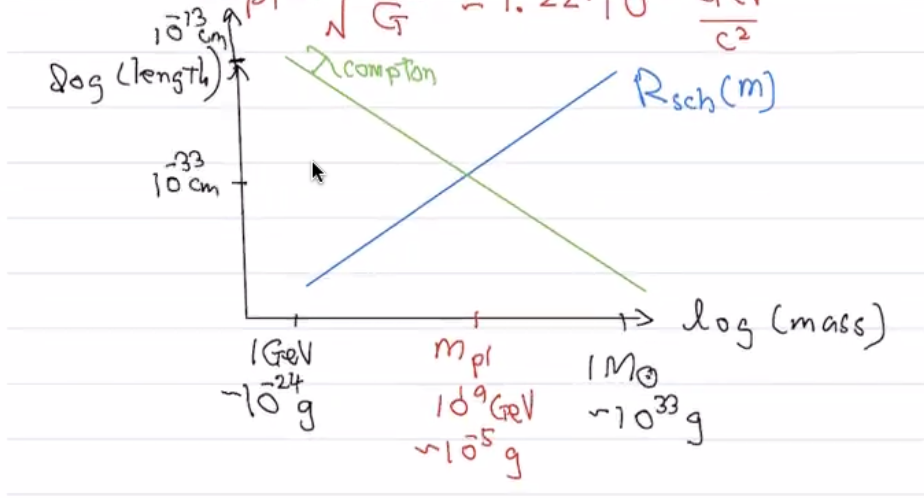
\includegraphics{scales.png}
    \caption{Length and mass scales, with the Planck mass being the intersection. }
    \label{fig:scales}
\end{figure}

A very natural scale for $\Lambda$ would be the Planck mass, right? Let's check that, looking at the Energy density in $\Lambda$ to order of magnitude:

\be
\Omega_\Lambda = 0.7 \approx 1 \rightarrow \rho_\Lambda \sim \rho_{c} \sim 1 \times 10^{-5} h^2 \frac{\unit{GeV}}{\unit{cm}^3}
\ee

Re-writing this with our conventions above (that $200 \unit{MeV} \approx \unit{fm}^{-1} \sim 10^{13} \cm^{-1}$. 

\be
\frac{1}{\cm^3} \sim \left(0.2 \unit{GeV}\right)^3\times 10^{-39} \sim 10^{-41} \unit{GeV}
\ee

Thus

\be
\boxed{\rho_\Lambda \sim 10^{-46} \unit{GeV}^4} 
\ee

Here comes the comparsion that should shock you. What's the natural scale, again? The Planck Scale! So how does $\rho_\Lambda$ compare with $m_\text{pl}^4$. 

\be
\boxed{m_\text{pl}^4 \sim 10^{76} \unit{GeV}^4}
\ee

Notice!

\be
\frac{\rho_\Lambda}{m_{pl}^4} \sim 10^{-122}
\ee

Why the heck is that so small? It's so ugly, unnatural, and not $\mathcal{O}(1)$.


\subsection{Thermodynamics in an Expanding Universe}


Here, we have lots of review of thermodynamics but applied to a non-static, fluid background. The conditions in the Early Universe (the first three minutes, or so). We had extremely high temperature, high pressure, and high density (either energy density $\rho$ or number density $n$). To a good approximation, though not always true, we have thermal equilibrium. Additionally, we can treat all these particles as if they are ideal gases -- gases where interactions are negligible. 

In phase space, we can have a phase space volume: $\mathrm{d}^3x \mathrm{d}^3 p$ which has units of $h_\text{planck}^3$. We use the term \textbf{phase space distribution function} $f(\vec{x},\vec{p},t)$, by the way. We thus have that:

\be
\text{Particle No.: } \mathrm{d}N = f(\vec{x},\vec{p},t) \frac{\mathrm{d}^3x \mathrm{ d}^3p}{h^3} g
\ee

When thermodynamics breaks down, we always can return to the evolution of $f$ directly, which is goverened by the \textbf{Boltzmann equation}. On a good day, we don't have to solve the 6-dimensional Boltzmann equation and can return to fluid dynamics instead. On a bad day, we have to return to our distribution function analysis. 

Now, recall from statistical mechanics: the equilibrium occupation number of a state of energy $\epsilon(p)$:

\be
f = \frac{1}{e^\frac{\epsilon-\mu}{kT} \pm 1}
\ee

where $+$ is for fermions  and $-$ is for bosons. Note as well that $\mu$ is the chemical potential:

\be
\mathrm{d}U =T \mathrm{d}S - P\mathrm{d}V + \mu \mathrm{d}N
\ee

The physical meaning of $\mu$ is thus the change in internal energy due to change in particle number! For a thermal radiation background, we have $\mu = 0$. This will be the case for most astrophysical contexts. 

The most obvious consequence of the above Boltzmann statistics is that the temperature evolves in time, but thermal equilibrium gives us spatial homogeneity. We need to know the first order perturbations to $f$ if we want to consider the non-linear Universe (the CMB!). 

Here are a few macroscopic, useful quantities:

\begin{itemize}
    \item Number density (where $\epsilon(p) = \sqrt{m^2 c^4 + p^2 c^2}$: 
    \be
    n = \frac{g}{h^3} \int_{0}^{\infty} \frac{4\pi p^2 }{e^\frac{\epsilon(p)}{kT} \pm 1}\mathrm{d}p
    \ee
    
    \item Energy density $u$:
    
    \be
    u = \rho = \frac{g}{h^3} \int_{0}^{\infty} \epsilon(p) \frac{4\pi p^2 }{e^\frac{\epsilon(p)}{kT} \pm 1}\mathrm{d}p
    \ee
    
    \item Entropy density $s$:
    \be
    s \equiv \frac{S}{V} = \frac{1}{V}\frac{1}{T} \left(U + PV - \mu N\right)
    \ee
    
    when $\mu = 0$:
    
    \be
    s = \frac{u+P}{T} 
    \ee
\end{itemize}


\noindent\textbf{Two limits:}
We will see familiar expressions when we take some limits. Starting with the \textbf{ultrarelativistic limit} $kT \gg mc^2$.\footnote{Note, again, that $T$ changes in time and therefore particles change from ultrarelativistic to non-relativistic throughout the evolution of the Universe. } Here, the particles are effectively massless and $\epsilon \rightarrow pc$. Computing these integrals:

\begin{itemize}
    \item Number density:
    \be
    n = \frac{g}{h^3}\int_0^\infty \frac{4\pi p^2}{e^{\frac{pc}{kT}} -1} \mathrm{d}p = \frac{4\pi g}{(2\pi)^3} \left(\frac{kT}{\hbar c}\right)^3 \int_0^\infty \frac{y^2}{e^{y} -1} \mathrm{d}y  
    \ee
    
    \item Energy density
    
    \be
    u = \frac{4\pi g}{(2\pi)^3}\left(\frac{k^4T^4}{\hbar^3 c^3}\right) \int_0^\infty \frac{y^3 \mathrm{d}y}{e^y \pm 1}
    \ee
    
    \begin{itemize}
        \item Bosons:
        
        \be
        n = \frac{1}{\Gamma(n)}\int_0^\infty \frac{y^{n-1} \mathrm{d}y}{e^y - 1}
        \ee
        
        We need two results:
        
        \be
        \int_0^\infty \frac{y^{2} \mathrm{d}y}{e^y - 1} = \Gamma(3) \zeta(3)
        \ee
        
        \be
        \int_0^\infty \frac{y^{2} \mathrm{d}y}{e^y - 1} = \Gamma(4) \zeta(4)
        \ee
        
        
        
        \item Fermions:
    \end{itemize}
\end{itemize}














\appendix 

\section{Archival Lectures (C.P. Ma)}

\subsection{Lecture 1}

\subsubsection{ The Cosmological Principle}

The {\bf Cosmological Principle} states that the universe is spatially 
{\it isotropic} (looks the same in all directions) 
and {\it homogeneous} (has constant density everywhere) on large scales.
The {\bf Perfect Cosmological Principle} states that the universe is
also {\it temporally} isotropic and homogeneous (a steady state universe). 
This is unlikely because it doesn't describe the Cosmic Microwave Background
(CMB).  The CMB and Hubble's Law are both provide evidence for isotropy and
homogeneity.

\subsubsection{ Hubble's Law (1929) }

Hubble's Law is an empirical law stating that, on large scales, recessional 
velocity is proportional to distance from observer.
$$\boxed{v=Hr}$$ 
where $H$, the Hubble parameter, is not constant, but can
vary slowly with time.  By convention, $H$ is often expressed as
$H=100\cdot h\frac{km}{ s\cdot Mpc}$, where 1 parsec (pc) $\approx3\cdot10^{18}cm
=3.26ly$, is the distance at which 1 AU appears as 1 arcsec on the sky.  
The Hubble Space Telescope Key Project (Freedman et al. ApJ 553, 47, 2001)
measured the present day value of Hubble Constant 
$H_0=72\pm 8\frac{km}{ s\cdot Mpc}$, giving us that the current timescale for
the expansion of the universe is 
$H_0^{-1}\approx\frac{h}{ 10^{11}}yrs\approx 9.778h^{-1}Gyrs$.

\subsubsection{ The Scale Factor }

$a(t)$ relates physical ($r$) and {\it comoving} ($x$) coordinates in an
expanding universe:
\begin{align}
r&=a(t)x\\
\dot r&=\dot ax+a\dot x=\underbrace{\aa}_{\equiv H}r+\underbrace{a\dot x}_{\equiv v_p}\\
\end{align}
Thus, the two components of physical velocity are $H$ (the Hubble expansion 
parameter) and $v_p$ (the peculiar velocity, or motion relative to expansion)
By convention, $t_0 \equiv$ today and $a(t_0)=1$.

\subsubsection{ The Friedmann Equations}

The Friedmann Equation is an equation of motion for $a(t)$.  A rigorous
derivation requires General Relativity, but we can fake it with a
quasi-Newtonian derivation.
We will model the universe as an {\it adiabatically} ($\Delta S=0$) expanding,
isotropic, homogeneous medium.  Isotropy allows us to use $r$ as a scalar.
Consider a thin, expanding spherical shell of radius $a$.
Birkhoff's Theorum states that even in GR,
the motion of such a shell depends only on the enclosed mass 
$M={4\pi }{ 3}a^3\rho$.
Thus, the energy per unit mass per unit length is:
$$E=\overbrace{\hf \dot a^2}^{Kinetic}\overbrace{-\frac{G\cdot M}{ a}}^{Potential}
=\hf \dot a^2-\frac{4\pi }{ 3}G\rho a^2.$$
We define $k\equiv-\frac{2E}{ c^2}$, and we will show later that $k$ is a measure
of the curvature of the universe: 
$$k\begin{cases}
>0&\,for\ E<0\ (bound)\\
=0&\,for\ E=0\ (critical)\\
<0&\,for\ E>0\ (unbound)\\\end{cases}$$
where $k$ has units of $\inv{length^2}$ if $a$ is dimensionless.  Substituting
$k$ into the above energy equation, and solving for $\aa$, we get:
\def\paap{\left(\aa\right)}
$$\boxed{H^2=\paap^2=\epot G\rho -\frac{k c^2 }{ a^2}}$$
\centerline{($1^{st}$ Friedmann Equation)}
This is a statement of conservation of $E$.
The first law of thermodynamics ($\Delta S=0$) requires that any 
system with positive pressure must lose energy as the volume enclosing it
expands.  Thus, if $U$ is our internal energy and $P$ is our pressure:
$$\frac{dU}{ dt}=-P\frac{dV}{ dt}.$$  
In an expanding universe, $U={E}{ V}\cdot V=\rho a^3$, where $\rho$ is the
energy density of the universe.  $P$ is the pressure of the photon gas, so:
$$\dot \rho a^3+3\rho a^2\dot a=-P 3a^2\dot a,$$ 
which simplifies to:
$$\boxed{\dot \rho=-3\aa(\rho +P)}$$
\centerline{($2^{nd}$ Friedmann Equation)}
This is a a statement of the temperature loss of the universe 
due to adiabatic expansion.\par
Finally, $\ddt$($1^{st}$ Friedmann Equation) gives us:
$$2\dot a\ddot a=\epot G \frac{d }{ dt}(\rho a^2) =\epot G a^2(\dot \rho +2\aa \rho).$$
Substituting the $2^{nd}$ Friedmann Equation for $\dot \rho$:
$$2\dot a\ddot a=\epot Ga^2 (-\aa \rho -3 \aa P) =-\epot G \aa (\rho +3P).$$  
Now we have our $3^{rd}$ Equation:
$$\boxed{\frac{\ddot {a }}{ a}=-\frac{4\pi G} {3} (\rho + 3P)}$$
\centerline{($3^{rd}$ Friedmann Equation)}
The $3^{rd}$ Friedmann Equation relates the acceleration of the expansion of
the universe to the pressure of photon gas and the density of the universe.
Note that if $3P \le -\rho$, we have an accelerating universe.\par
Compare the $3^{rd}$ Friedmann Equation to the Newtonian equation for gravity,
with $M=\frac{4\pi }{ 3}\rho x^3$ and $\rho_{eff}=\rho +3P$:
$$\ddot x=\frac{-G\cdot M}{ x^2}={-4\pi }{ 3}G\rho x$$

\subsection{Lecture 2}

\subsubsection{ The Friedmann Equations, continued }

Recall we had the following equations:
$$\paap^2={8\pi}{3}G\rho-\frac{k}{ a^2}$$
$$\dot \rho=-3\aa(\rho+P)$$
$$\frac{\ddot a}{ a}=-\frac{4\pi}{3}G(\rho+3P)$$

To close the equations, we need to relate $P$ and $\rho$ with an equation of
state:
$$\boxed{P=w\rho(c^2)}$$ 
Note that we will generally set $c=1$ in this class.
Combined with (2), this gives us:
\begin{align}
\dot \rho&=-3\aa(1+w)\rho\\
{\dot \rho}{\rho}&=-3(1+w)\aa\\
\rho&\propto\atow\\
\end{align}
Note that we've assumed $\dot w=0$, which is okay most of the time.
Some special cases of interest are:
\begin{itemize}
\item Pressure-less ``dust'' $P=0$, $w=0\imply\rho\propto a^{-3}$ because volume
goes as $V\propto\inv{a^3}$.
\item Relativistic particles (photons, bosons): $w=\inv{3}$, $P=\frac{\rho}{3}
\imply\rho\propto a^{-4}$ because $VV\propto\inv{a^3}$, and energy is given
by $E\propto\inv{a}$.
\item  ($\Lambda$)/Dark Energy: $w=-1$, $P=-\rho\imply\rho=$ constant 
in time.
\end{itemize}
To get density ($\rho$) as a function of time, want to solve for $w$.

\subsubsection{ Critical Density}

We define $\rho_{crit}$ to be the critical density at which $k=0$ (and $E=0$):
\def\rcr{{\rho_{crit}}}
$$\rcr=\frac{3H^2}{8\pi G}$$
Today, we measure: $\rho_{crit,0}=\frac{3H_0^2}{8\pi G}= 
\frac{3}{8\pi}\frac{\left(100h\frac{km}{ sMpc}\right)^2}{ G}=2.78\cdot10^{11}h^2
\frac{M_\odot}{ Mpc^3}=1.88\cdot10^{-29}h^2\frac{g}{ cm^3}$.
Note that the mass of the sun is $M_\odot=2\cdot10^{33}g$, and
the mass of the proton is $M_p=1.67\cdot10^{-24}g$.

\subsubsection{ Density Parameter}

$\Omega$ measures the ratio of the density of the universe to the critical
density:
$$\Omega(t)\equiv\frac{\rho(t)}{\rho_c(t)}=\frac{8\pi G\rho(t)}{ 3H^2(t)}$$
$$\Omega\begin{cases}
\le1&\imply open\ (k\le0)\\
=1&\imply flat\ (k=0)\\
\ge1&\imply closed\ (k\ge0)
\end{cases}$$

In general, $\Omega$ can consist of multiple components: 
$\Omega=\sum_i{\Omega_i}$ e.g. 
$$\Omega\begin{cases}
r&=radiation\\ 
m&=matter\ (dark\ and\ luminous)\\
b&=baryons\ (dark\ and\ luminous)\\ 
\nu &=neutrinos\\ 
\Lambda&=dark\ energy\end{cases}$$

$\Omega = 1$ is an unstable equilibrium; any perturbation from $\Omega=1$ in
the early universe ensures $\Omega$ is far from 1 today.  That we measure
$\Omega_m\approx0.3$ today implies that the early universe must have been
extremely finely tuned.

\subsubsection{ Evolution of Hubble Parameter}

Today (at $a=1$): $k=\epot G\rho_0-H_0^2=H_0^2(\Omega_0-1)$.  Using the
$1^{st}$ Friedmann equation (1), we have:
$$\boxed{H^2=H_0^2(\frac{\Omega_0}{ a^{3+3w}}+\frac{1-\Omega_0}{ a^2})}$$
\centerline{\bf (THE Friedmann Equation)}
where $H_0\equiv\sqrt\frac{8\pi G\rho}{3\rcr}$, and it is understood that
$\etot=\sum_i{\Omega_{i,0}}$.  Each $\Omega_i$ has it's own $w_i$, so really
$\frac{\Omega_0}{\attw}=\sum_i\frac{\Omega_{i,0}}{ a^{3+3w_i}}$.

\subsubsection{ Evolution of Density Parameter}

We'll show in PS\#1 that for any single component:
$$\frac{1-\Omega(a)}{\Omega(a)}=\frac{1-\Omega_0}{\Omega_0}a^{1+3w}$$
Plotting $\Omega(a)$, we will find that for early $a$, $\Omega$ is {\it 
extremely} close to 1.

\subsubsection{ Evolution of Scale Factor: Solving the Friedmann Equation}

The evolution of the expansion of the universe is governed by:
$$\paap^2=\epot G\rho-\frac{k}{ a^2}$$

We can apply this to several models of the universe:
\begin{itemize}
\item The Einstein-deSitter (flat) Model: $k=0$, $\Omega(a)=\Omega_0=1$.
Using that $\rho\propto\atow$, we have:
\begin{align}
\paap^2&\propto\atow\\
a^{-1}a^{\frac{3}{ 2}(1+w)}da&\propto dt\\
\athow&\propto t\\
\end{align}$$
$$\boxed{a(t)\propto t^{\frac{2}{ 3(1+w)}}}
Thus, the rate of expansion of the universe depends on $w$:
\item{(a)} The matter-dominated era: 
$\Omega\approx\Omega_m\imply w=0, P=0, a\propto t^\frac{2 }{ 3}$.
\item{(b)} The radiation-dominated era: 
$\Omega\approx\Omega_r\imply w=\inv{3} \imply a(t)\propto t^\hf$.
\item{(c)} The $\Lambda$-dominated era: 
$\Omega\approx\Omega_\Lambda\imply w=-1, P=-\rho, \rho$ constant in time
$\imply a(t)\propto e^{Ht}$, where H is now actually a constant.  This
is exponential inflation.  We used to think that this only happened early on 
(like $10^{-34}$
seconds), but now we think that this has also been happening recently.
Next time, we will do the harder two cases: open and closed.
\end{itemize}

\subsection{Lecture 3}

\subsubsection{ Evolution of Scale Factor: Solving the Friedmann Equation, continued }

Last time we did (1), the flat universe:

Einstein-deSitter, $k=0$ (flat), $\Omega =1,\imply$
 $a\propto t^\frac{2}{ 3(1+w)}$. In general, we consider the evolution of
the universe to be {\it matter dominated} if $a\propto t^\frac{2}{ 3}$,
{\it radiation dominated} if $a \propto t^{\hf}$, and 
{\it $\Lambda$ dominated} if $a \propto e^{1+t}$ (that is, $H$ is constant).


Open, $k<0$, $\etot<1$, $\econs=0$, $\emat<1\imply$ our Friedmann
Equation $\paap^2=\epot G\rho-\frac{k}{ a^2}$ becomes:
$$\dot a^2=H_0^2\left(\frac{\etot }{ a^{1+3w}}+1-\etot\right)$$  
Since we are matter dominated, $w=0$.  Solving for $a(t)$:
\begin{align}
\int_0^{a_f}\frac{da}{\sqrt{{\etot}{ a}+1-\etot}}
&=\int_0^{t_f}{H_0\cdot dt}\\
\int_0^{a_f}\frac{a\cdot da}{\sqrt{1-\etot}\sqrt{a^2+\frac{\etot}{1-\etot}a}}
&=H_0t_f\\
\end{align}
Let's define $2\alpha\equiv\frac{\etot}{1-\etot}$.  Then:
$$\int_0^{a_f}\frac{a\cdot da}{\sqrt{1-\etot}\sqrt{(a+\alpha)^2-\alpha^2}}
=H_0t_f$$
Defining $a^\prime=a+\alpha$, we get:
\begin{align}
\int_0^{a_f+\alpha}\frac{(a^\prime-\alpha)da^\prime}{ 
\sqrt{1-\etot}\sqrt{a^{\prime 2}-\alpha^2}}&=H_0t_f\\
\int_0^{a_f+\alpha}\frac{(a-\alpha)da}{ \sqrt{1-\etot}\sqrt{a^2-\alpha^2}}
&=H_0t_f\\
\end{align}
Now we define $\alpha\cosh\theta\equiv a^\prime$, 
$\alpha\sinh\theta\,d\theta=da$, so that 
$\sqrt{a^{\prime 2}-\alpha^2}=\alpha\sinh\theta$.  We'll be lazy and
just say that $a_f^\prime\to\frac{\etot }{ 2(1-\etot)(\cosh\theta -1)}$ because
there was nothing special about time $a_f^\prime$. Then we have:
\begin{align}
\int_0^{\theta_f}\frac{\alpha^2(\cosh\theta-1)\sinh\theta\,d\theta}{
\sqrt{1-\etot}\alpha\sinh\theta}&=H_0t_f\\
\frac{\alpha}{1-\etot}(\sinh\theta-\theta)\bigg|_0^{\theta_f}&=H_0t_f\\
\end{align}

Plugging $\alpha$ back in:
\begin{align}
H_0t_f&=\frac{\etot}{2(1-\etot)^\frac{3}{ 2}}(\sinh\theta-\theta)\\
t(\theta)&=\frac{\etot}{2H_0(1-\etot)^\frac{3}{2}}(\sinh\theta-\theta)\\
\end{align}
Thus we have a parametric relationship between $a$ and $t$ with a dummy
variable $\theta$:
\begin{align}a(\theta)&=\frac{\etot}{ 2(1-\etot)}(\cosh\theta-1)\\
t(\theta)&=\frac{\etot}{ 2\,H_0(1-\etot)^{3}{ 2}}(\sinh\theta-\theta)\\
\end{align}
Note that $a$ has no maximum and expands forever.

Closed, $k>0$, $\etot>1$, $\Omega_\Lambda=0$. As usual,
we start with the Friedmann Equation:
$$(\aa)^2 = \underbrace{\overbrace{\epot G\rho}^{positive} - 
\overbrace{\frac{k}{ a^2}}^{positive}}_{can\ be\ 0}$$
Therefore, in this model it is possible for $\dot a=0$.  We'll again solve for a
matter-dominated era, $w=0$.  The solution is similar, to the open model, 
but ($1-\etot<0$), so $\theta\to i\,\theta$. Thus our solution:
\begin{align}a(\theta)&=\frac{\etot}{ 2(1-\etot)}(\cos\theta-1)\\
t(\theta)&=\frac{\etot}{2H_0(1-\etot)^\frac{3}{ 2}}(\sin\theta-\theta)\\
\end{align}
is a cycloid solution.  That is, $a$ oscillates, with a maximum at 
$\theta=\pi$.

\subsubsection{ Deceleration Parameter q}

$$q\equiv-{\ddot aa}{ \dot a^2}$$
Note that $q$ is {\it dimensionless}, and has a negative sign.  The minus is
there because historically, the universe was thought to be decelerating.  Thus,
$q<0\imply acceleration$, and $q>0\imply deceleration$.  We can find out what
$q$ does from the $2^{nd}$ Friedmann Equation:
$$\adda=-\frac{4\pi}{3}G(\rho+3P)$$
Recall that $P=w\rho$, $\Omega=\frac{\rho}{\rcr}$,
$\rcr=\frac{3H^2}{8\pi G}$, $H^2\Omega=\epot G\rho$. Thus, the
above equation becomes:
$$\adda=-\frac{4\pi}{3}G\rho(1+3w)=-\frac{H^2\Omega}{2}(1+3w)$$
Substituting in our friend, $q$:
$$q=\frac{\Omega}{2}(1+3w)=\sum_i{\frac{\Omega_i}{2}(1+3w_i)}$$
$$\boxed{q = \frac{\Omega _m }{ 2} - \Omega _\Lambda +\Omega _r}.$$
Note that today, $\Omega_r\ll1$.  That we are accelerating $\imply q<0
\imply\econs\ne0$.

\subsubsection{ Redshift }

$$\frac{\lambda_{obs} }{ \lambda_{emit}} \equiv 1 + z$$
Or alternately,
$$\boxed{1 + z = \frac{1}{ a}}$$
$z$ is what we call the {\it redshift}. Reionization happened somewhere
around $z=17\pm6$, and recombination around $z=1091$.

\subsubsection{ Time-Redshift Relations and the Age of the Universe }

We seek a relation between $t$ and $z$.  Beginning with the Friedmann Equation:
\begin{align}
H^2&=H_0^2\left[\jumble\right]\\
\inv{a}\frac{da}{ dt}&=H_0\sqrt{\jumble}\\
dt&=\inv{H_0}\left(\inv{a}\right)\frac{da}{\sqrt{\jumble}}\\
dt&=-\inv{H_0}\frac{dz }{ (1+z)\jimble}\\
\end{align}
We can calculate the time since the Big Bang at redshift $z_1$ by solving the
integral:
$$t_1=-\inv{H_0}\int_{z_1}^\infty{\frac{dz}{ 1+z}\inv{\jimble}}$$
For the Age of the Universe, set $z_1=0$.  In the special case of a flat
(Einstein-deSitter) universe: 
$$t_0=\inv{H_0}\int_0^\infty\frac{dz}{(1+z)^\frac{5}{ 2}}={2}{3H_0}$$  
If $H_0^{-1}\approx10Gyrs$,
then $t_0\approx6.7h^{-1}Gyrs$, so the Hubble constant needs to be pretty
small to get reasonable estimates of the age of the universe.



\subsection{Lecture 4}

\subsubsection{ Time-Redshift Relations and the Age of the Universe }

Last time we found the age of a flat universe.
in a flat (Einstein-deSitter) universe: 
$k=0$, $\Omega_m=1$, $\Omega_\Lambda=0$, so:
$$t_0=\inv{H_0}\int_0^\infty{\frac{dz}{(1+z)^\frac{5}{ 2}}}
=\frac{2}{3H_0}\approx6.7h^{-1}Gyr$$
Alternatively, recall that for a matter-dominated era,
$a(t) = ({t}{ t_0})^\frac{2}{ 3}.$
Thus, $H = \aa = \frac{2}{ 3t} \imply t_0=\frac{2}{ 3H_0}$.

If we have $\Lambda\ne0$: $k=0$, $\emat+\econs=1$, then:
$$t_0=\inv{H_0}\int_0^\infty\frac{dz}{(1+z)\sqrt{\emat(1+z)^3+\econs}}$$
Assuming $0.1\le\emat\le1$, this integral is solvable:
$$t_0=\frac{2}{3H_0}\inv{\sqrt{1-\emat}}\ln\left(\frac{1+\sqrt{1-\emat}}{
\sqrt{\emat}}\right)\approx\frac{2}{3H_0}(0.7\emat+0.3-0.3\econs)^{-0.3}
\approx\frac{2}{3H_0}\emat^{-0.3}$$
Generally, in a flat universe, $t_0\propto\inv{H_0}$.  If $\Omega_0\le1$, 
it will be longer.

In an open universe: $k<0$, $\etot<1(\econs=0)$. Recall:
$$\begin{matrix} t(\theta)=\frac{\etot}{2H_0(1-\etot)^\frac{3}{2}}(\sinh\theta-\theta),&
a(\theta)=\frac{\etot}{2(1-\etot)}(\cosh\theta-1)\end{matrix}$$

So today: 
\begin{align}
a(\thnot)&={\etot}{ 2(1-\etot)}(\cosh\thnot -1)=1\\
\cosh\thnot&=\frac{2(1-\etot)}{\etot}+1=\frac{2-\etot}{\etot}\\
\sinh\thnot&=\sqrt{\cosh^2\thnot-1}=\frac{2}{\etot}\sqrt{1-\etot}\\
t_0&=t(\thnot)-\frac{\etot}{ 2H_0(1-\etot)^\frac{3}{ 2}}\left[\frac{2}{\etot}
\sqrt{1-\etot}-\cosh^{-1}\left(\frac{2-\etot}{\etot}\right)\right]\\
\end{align}

$$\boxed{t_0=\inv{H_0}\left[(1-\etot)^{-1}-\hf(1-\etot)^{-\frac{3}{ 2}}
\cosh^{-1}\left(\frac{2-\etot}{\etot}\right)\right]}$$

Thus $t_0>\frac{2}{ 3H_0}$ for $\etot\le 1$, and $t_0=\inv{H_0}$ for $\etot=0$
(an empty universe).

In a closed universe: $k>0$, $\etot>1$, $(\econs=0)$. Recall: 
\begin{align}
t(\theta)&=\frac{\etot}{ 2H_0(\etot -1)^\frac{3}{2}}(\theta-sin\theta)\\
a(\theta)&=\frac{\etot}{ 2(\etot -1)}(1-\cos\theta)\\
\end{align}

Thus, today:
$$a(\theta_0)=\frac{\etot}{ 2(\etot -1)}(1-\cos\theta)=1$$
$$\boxed{t_0=\inv{H_0}\left[(1-\etot)^{-1}+\hf\etot(\etot-1)^{-\frac{3}{ 2}}
\cos^{-1}\left(\frac{2-\etot}{\etot}\right)\right]}$$

\subsubsection{ The Robertson-Walker Metric}

Lorentz invariance dictates that two inertial
frame $(x, y, z, t)$ and $(x\p, y\p, z\p, t\p)$, with one 
moving with respect to the other at velocity $\hat v=v\hat x$, are related by:
$$\begin{matrix} x\p=\gamma(x-vt),&y\p=y,&z\p=z,&t\p=\gamma\left(t-\frac{v}{ c^2}x
\right)\end{matrix}$$
where $\gamma\equiv\frac{1}{\sqrt{1-\frac{v^2}{ c^2}}}$.  
Note, to give a taste of tensor forms, this all
may be written as ${x\p}^\alpha = \Lambda^\alpha_\beta x^\beta+I_0^\alpha$.\par

Remember the Lorentz invariant interval, which is conserved between frames:
$$ds^2=c^2dt^2-(dx^2+dy^2+dz^2)$$
Light travels a $ds^2=0$ path.  In tensor form, this equation looks like:
$$ds^2=g_{\alpha\beta}dx^\alpha dx^\beta$$
where $g_{\alpha\beta}$, the metric tensor, is given by:
$$g_{\alpha\beta}\equiv\begin{pmatrix} 1&0&0&0\\0&-1&0&0\\0&0&-1&0\\ 0&0&0&-1\\
\end{pmatrix}$$
Look at Weinberg, Ch. 13 for full proof, but for a homogeneous, 
$\gamma$-isotropic space, the metric looks like: 
$$ds^2=c^2dt^2-a^2(t)\left[\frac{dr^2}{ 1-kr^2}+r^2d\Omega\right]$$
where $r$ is a radial direction (in
comoving coordinates), and $d\Omega=d\theta^2+\sin^2\theta d^2\phi$ is the
differential angle seperation of two points in space.  As usual,
$k$ is the measure of curvature.


The $k=0$ Model: 
$$dr^2+r^2(d\theta^2+\sin^2\theta d\phi^2)=dx^2+dy^2+dz^2$$
so we recover the Minkowski metric for flat space, using comoving coordinates.

The $k>0$ (closed) Model:\par
We get a coordinate singularity at $r=\frac{1}{\sqrt{k}}$, so this universe
has a finite volume.
For $k>0$, we need to define ``Polar Coordinates'' in 4-D (to describe a
3-sphere embedded in 4-D).  Here is a comparison of how we define polar 
coordinates for a 3-sphere in 4-D versus for a 2-sphere in 3-D:
$$\begin{matrix} 
3-sphere&2-sphere\\
(x,y,z,w)\iff (R,\alpha,\beta,\gamma)&(x,y,z)\iff(R,\theta,\phi)\\
w=R\cos\alpha&z=R\cos\theta\\
z=R\sin\alpha\cos\beta&y=R\sin\theta\cos\phi\\
y=R\sin\alpha\sin\beta\cos\gamma&x=R\sin\theta\sin\phi\\
x=R\sin\alpha\sin\beta\sin\gamma& \\
x^2+y^2+z^2+w^2=R^2&x^2+y^2+z^2=R^2\\
\end{matrix}$$

Take a line element on a 2-sphere: 
$$d\gamma=R^2(d\theta^2+\sin^2\theta d\phi^2)$$
Changing variables for $v\equiv\sin\theta$:
$$dv=\cos\theta d\theta=\sqrt{1-v^2}d\theta$$
Then $d\theta^2=\frac{dv^2}{1-v^2}$, so rewriting our line element, we get:
$$d\gamma^2=R^2\left(\frac{dv^2}{ 1-v^2}+v^2d\phi^2\right)$$
For a 3-sphere, 
$$d\gamma^2=R^2(d\alpha^2+\sin^2\alpha d\Omega^2)$$
where $d\Omega^2\equiv d\beta^2+\sin^2\beta d\gamma^2$.  Again, using a change
of variables so that $v\equiv\sin\alpha$, $d\alpha=\frac{dv}{\sqrt{1-v^2}}$,
we get that:
$$\boxed{d\gamma^2=R^2\left(\frac{dv^2}{ 1-v^2}+v^2d\Omega^2\right)}$$
This is what Robertson-Walker showed. 


\subsection{Lecture 5}

\subsubsection*{ Finishing the Robertson-Walker Metric}

We've been following Weinberg's derivation to show there are discrete metrics.
We'll start with:
$$ds^2=c^2dt^2-a^2(t)\left[\frac{dr^2}{ 1-kr^2}+r^2(d\theta^2+\sin^2\theta 
d\phi^2)\right]$$
Recall that $k$ is the {\it curvature constant} and $r$ is in {\it comoving}
coordinates.  If we define $U\equiv\sinh\theta$, then: 
\begin{align}
dU&=\cosh\theta\cdot d\theta\\
d\theta&=\frac{dU}{\sqrt{1+U^2}}\\
\end{align}
The beauty of this metric
is that we derived it only using symmetry (no dynamics).  There is an alternate
way of writing the metric above:
$$ds^2=c^2dt^2-a^2
\left[d\chi^2+S^2(\chi)(d\theta^2+\sin^2\theta d\phi^2\right]$$
where:
$$S(\chi)\equiv\begin{cases}\chi &\,(for\ k=0,\ \chi=r)\\
k^{-\hf}\sin(k^\hf \chi)&\,(for\ k>0)\\
(-k)^{-\hf}\sinh(\sqrt{-k}\chi)&\,(for\ k<0)\\\end{cases}$$
\par

\subsubsection*{ Comoving Radial Distance vs. Redshift: the Hubble Diagram }

This is the fundamental diagram behind using a standard candle (supernova) to
infer the curvature of the universe.  What we want here is an algebraic
expression relating $r$ and $z$.  We'll look at light propagation ($ds^2=0$),
and take a radial path ($d\theta=d\phi=0$) to know from the Robertson-Walker
metric that:
$$c^2dt^2=a^2\frac{dr^2}{1-kr^2}$$
Separating out our $r$ dependencies
and our $t$ dependencies and integrating, we get:
$$\int_0^{r_1}\frac{dr}{\sqrt{1-kr^2}}=\int_{t_1}^{t_0}\frac{c\cdot dt}{ a(t)}$$
\begin{itemize}
\item For the flat, $k=0$, matter-dominated model ($w=0$, $\econs=0$, 
$\emat=1$), we'll start with the Friedmann Equation:
$$H=\aa=H_0\sqrt{\frac{\etot}{\attw}+\frac{1-\etot}{ a^2}}$$
Recognizing that $a=\inv{1+z}$, we have:
$$H_0dt=-\frac{dz}{ (1+z)\sqrt{\etot(1+z)^{3+3w}+(1-\etot)(1+z)^2}}$$
These integrals evaluate to (in comoving $r$):
$$r_1=\int_{t_1}^{t_0}\frac{c\cdot dt}{ a(t)}$$
$$\boxed{r_1=\frac{2c}{ H_0}\left[1-(1+z)^{-\hf}\right]}$$
\def\hubd{\frac{2c}{ H_0}}
\def\sqmk{\sqrt{-k}}
Here, $\hubd$ is called the Hubble distance and is the definition of 
how far away we can possibly see--how far light could have traveled since the
beginning of time.  Notice that as $z\to\infty$, $r=\hubd\approx10000h^{-1}Mpc$.

\item For the open, $k<0$, $\etot<1$, $w=0$ model, we'll substitute 
$\sqmk r=\sinh\chi$, $dr=\frac{\cosh\chi d\chi}{\sqmk}$ for $r$ in the integral 
above:
\begin{align}
r&=\int_-^{\chi_1}\frac{\cosh\chi d\chi}{\sqmk\sqrt{1+\sinh^2\chi}}\\
\frac{\chi_1}{\sqmk}&={\sinh^{-1}(\sqmk r_1)}{\sqmk}\\
\end{align}
From this, we can use {\it Mattig's Formula}, which states for $w=0$, 
arbitrary $\emat = \etot$, that:
$$r=\frac{2c}{ H_0\etot^2}\inv{1+z}\left[\etot z+(\etot-2)(\sqrt{1+\etot z}
-1)\right]$$
In general, for arbitrary $\emat, \econs$ (we'll derive this in PS\#3), one
can show that, in comoving $r$:
\def\sqak{\sqrt{|k|}}
$$
\boxed{r=\inv{\sqak}sinn\left(\frac{c}{ H_0}\sqak 
\int_0^z\frac{dz\p}{ \sqrt{\emat(1+z)^3+\econs+(1-\emat-\econs)(1+z)^2}}
\right)}$$
where $sinn$ is a funny function: 
$$sinn\equiv\begin{cases}\sin&\,for\ k>0\\
absent&\,for\ k=0\\
\sinh&\,for\ k<0\\\end{cases}$$
Note that when $w=0$, for arbitrary $\emat$, we recover Mattig's Formula.
\end{itemize}

\subsubsection*{ Angular Diameter Distance}

The angular diameter distance is a useful quantity which relates the physical
size or separation of objects to the angular size on the sky.  For normal,
Euclidean geometries, this is trivial trigonometry.  For a curved universe,
this is not trivial.  For example, in some universes, an object pulled
far enough away may actually start looking larger (have a larger angular
diameter) than a closer object!\par
This brings us to the end of the smooth universe.  We've seen $a(t)$, but we
have not seen any perturbations off of that.  Similarly, we've seen $\rho (t)$,
but no spatial components of density.  We will begin to talk about perturbations
off of the Smooth Universe, and we will call this:

\subsubsection*{ The Bright Side of the Universe}

Let's do a quick tour of the the particles out there to give some context
to what we're talking about.  Take a look at {\it Review of Particle Physics},
which is also at {\it http://pgd.lbl.gov}, for some more detailed information.
\par
First, we'll talk about {\it fermions}.  Fermions come in two varieties:
Leptons and Quarks.  Quarks are hadrons and group together to from
baryons (made of 3 quarks) and mesons (made of quark-antiquark pairs).
\centerline{Elementary Particles: Fermions (spin $\hf$)}
$$\begin{matrix} 
Leptons&Charge&Mass&Mean\ Lifetime\\
e&-1&0.51099892\pm0.00000004 MeV&\infty\\
\nu_e&0&<3 eV&\infty\\
\mu&-1&106 MeV&2.2\mu s,\ \mu^-\to e^-\bar \nu_e\nu_p\\
\nu_\mu&0&<190 keV&\infty\\
\tau&-1&1.78 GeV&2.9\cdot 10^{-13}\\
\nu_\tau&0&<18.2 MeV&\infty\\\end{matrix}$$

$$\begin{matrix} 
Quarks\ (3\ colors\ each)&Charge&Mass\\
U&\frac{2}{ 3}&1.5 \to 4 MeV\\
d&-\frac{1}{ 3}&4 \to 8 MeV\\
s&-\frac{1}{ 3}&80 \to 130 MeV\\
c&\frac{2}{ 3}&1.15 \to 1.35 GeV\\
b&-\frac{1}{ 3}&4.1 \to 4.4 GeV\\
t&\frac{2}{ 3}&174.3 \pm 5.1 GeV\\\end{matrix}$$


\subsection{Lecture 6}

\subsubsection*{ The Bright Side, continued }

$$\begin{matrix} 
Gauge\ Bosons&spin&charge&mass\\
\gamma&1&0&0&(carries\ electroweak\ force)\\
w^\pm&1&\pm 1&80.4 GeV&(carries\ electroweak\ force)\\
Z^0&1&0&91.2 GeV&(carries\ electroweak\ force)\\
gluons&1&0&don't\ know&(carries\ strong\ force)\\
Higgs&0&0&>114.4GeV\\
graviton&2&0&0\\\end{matrix}$$

$$\begin{matrix} 
Baryons&quark\ content&charge&mass&lifetime\\
proton&uud&+1&938.07003 MeV&\ge 10^{32} yrs\\
neutron&udd&0&939.56536 MeV&885.7 sec\\
\Lambda&uds&0&1.11 GeV&10^{-10} sec\\
\Sigma^{+,0,-}&uus,uds,dds&+1,0,1&1.2 GeV&10^{-10}, 10^{-19}\\
\Xi^0&uss&0&1.3 GeV&10^{-10}\\
\Xi^-&dss&-1&1.3 GeV&10^{-10}\\
\Omega^-&sss&-1&1.67 GeV&?\\\end{matrix}$$

$$\begin{matrix} 
Mesons(q\bar q,\ Spin\ 0)&charge&quark&mass&lifetime\\
\Pi^\pm&\pm 1&u\bar d, d\bar u&140MeV&10^{-8}s\\
\Pi^0&0&u\bar u, d\bar d&135MeV&10^{-16}s\\
K^\pm&\pm1&u\bar s,\bar us&494 MeV&10^{-8} s\\
(Spin\ 1)\\
J,\Psi&0&c\bar c&3.1 GeV&10^{-20}\\
\Upsilon&0&b\bar b&9.5 GeV&10^{-20}\\\end{matrix}$$

$$\begin{matrix} 
Fundamental\ Interactions&Gravity&Weak&EM&Strong\\
Classical&Newton/Einstein&-&Maxwell&-\\
Quantum&?&V-A\ Theory(flawed)&QED, Gauge&QCD [SU(3)]\\\end{matrix}$$

\subsubsection*{ Useful Scales/Conversion tricks}

In particle physics, $E\sim\inv{length}$, because $\hbar c=1$ (which
had units $\frac{E}{ cm}$).  In condensed matter physics, $E\sim T$.\par
The Planck mass is the mass scale at which the effect of gravity and quantum
effects are comparable.  We can get an estimate of the Planck mass by setting
the Schwarzschild radius ($R_{sch} = \frac{2Gm}{ c^2}$) equal to the Compton
wavelength of a particle ($\lambda = \frac{hc}{ mc^2} = \frac{2\pi\hbar c}{ mc^2}$).
Dropping our constants (2's, $\pi$'s), we get:
$$\frac{Gm_{planck}}{ c^2} \sim \frac{\hbar c}{ m_{planck}c^2}$$
$$m_{planck} = \sqrt{\frac{\hbar c}{ G}} \approx 1.2\cdot 10^{19} \frac{GeV}{ c^2}$$
Another number of interest is the energy density in $\Lambda$.  We know
$$\econs \equiv \frac{\rho_\Lambda}{ \rho_{crit}} \approx 0.7 \sim 1$$
\begin{align}
\rho_\Lambda \sim \rho_{crit} 
&= 1.88\cdot 10^{-29} h^2 \frac{g}{ cm^3}\\
&= 1.054\cdot 10^{-5} h^2 \frac{GeV}{ cm^3}
\end{align}
Converting $\frac{GeV}{ cm^3}$ to $GeV^4$, we get:
$$\rho_\Lambda \sim \rho_{crit} \sim 10^{-46} GeV^4$$
$$\frac{\rho_\Lambda}{ m_{planck}^4} \approx 10^{-122} = worst\ number\ in\ 
physics$$

\subsection{Lecture 7}

The lower the temperature of the universe, the easier life gets: once the 
temperature of the universe drops below the rest energy of a particle, it is
no longer often created in particle/antiparticle pairs.\par

\subsubsection*{ Thermodynamics of a Fermi/Bose Gas}

{\it Phase Space} is a 6-dimensional space of directions and linear momenta.
It has volume:
$$V = {d^3xd^3p\over h^3}$$
The {\it Distribution Function} $f(\hat x,\hat p,t)$ describes the number of particles
in a particular $\hat x, \hat p$ state at a given time.  Thus, the number of particles
in a phase space volume is:
\def\fxpt{f(\hat x,\hat p,t)}
$$dN=f(\hat x,\hat p,t){d^3xd^3p\over h}\cdot g$$
where $g$ is used to account for {\it degeneracy}.
Reminder of Fermi/Bose statistics:
\def\eeukt{e^{E-\mu\over kT}}
$$\fxpt = \inv{\eeukt\pm 1}$$
Where $\mu$ is the chemical potential (usually 0 for us), + is for fermions,
and - is for bosons.  The chemical potential is usually 0 because we are talking
about photons, and it can be shown that since photon number is not conserved,
then $\mu = 0$.  
\begin{itemize}
\item \# density in thermal equilibrium (integrating $dN$ above, dividing
by volume, recall $E=\sqrt{p^2c^2+m^2c^4}$):
$$n = {g\over h^3}\int{4\pi p^2dp\over e^{E(p)\over kT}\pm 1}$$
\item Energy density ($dN$, weighted by energy):
$$u={g\over hA^3}\int_0^\infty{E(p){4\pi p^2dp\over e^{E(p)\over kT}\pm 1}}$$
\item Entropy density $s={S\over V}=\inv{V}\inv{T}(U+PV-\mu N)$.  $P$ is
pressure. For $\mu=0$:
$$s={u+P\over T}$$
Without proving, we'll state $P=\langle{p^2c^2\over 3E}\rangle$.  
The proof comes from
kinetic theory.  Thus:
\def\epkt{e^{E(p)\over kT}}
$$s={g\over h^3}\int_o^\infty{{4\pi p^2dp\over\epkt\pm 1}\left({E(p)\over T}
+{p^2c^2\over 3ET}\right)}$$
\end{itemize}
So we have ways to calculate 3 very useful quantities for the early universe.  
We can take two useful limits of these quantities:

\subsubsection*{ Ultra-relativistic ($kT\gg mc^2$) Particles in the Early Universe }

In this limit, particles are effectively massless (their energy is 
dominated by their motion, $E=\sqrt{m^2c^4+p^2c^2}\approx pc$).  
\begin{itemize}
\item"A." Bosons
\item{(1)} The \# density of relativistic bosons is:
\begin{align}
n&={g\over h^3}\int_0^\infty{4\pi p^2dp\over e^{pc\over kT}\pm 1}\\
&={4\pi g\over (2\pi)^2}\left({kT\over \hbar c}\right)^3
\int_0^\infty{y^2dy\over e^y\pm 1}\\
\end{align}
where $y\equiv {pc\over kT}$.  This integral is calculable, and is the 
definition of the Reimann-Zeta function:
\begin{align}
\zeta(n)&\equiv\inv{\Gamma(n)}\int_0^\infty{y^{n-1}dy\over e^y-1}\\
\int_0^\infty{y^2dy\over e^y-1}=\Gamma(3)\zeta(3)&\approx 2\cdot 1.202\\
\int_0^\infty{y^3dy\over e^y-1}=\Gamma(4)\zeta(4)&={\pi^4\over 15}\\
\end{align}
So getting back to the \# density of bosons:
$$\boxed{n_B={g\over\pi^2}\zeta(3)\left({kT\over\hbar c}\right)^3}$$

\item{(2)} The energy density of relativistic bosons is:
\def\epckt{e^{pc\over kT}}
\begin{align}
u&={g\over h^3}\int_0^\infty{pc{4\pi p^2dp\over\epckt\pm 1}}\\
&={4\pi g\over (2\pi)^3}{(kT)^4\over(\hbar c)^3}
\int_0^\infty{y^3dy\over e^y\pm 1}\\
\end{align}$$
$$\boxed{u_B={\pi^2\over 30}g{(kT)^4\over(\hbar c)^3}}
For photons, $g=2$.  We can calculate a flux related to their energy density:
$$F=\inv{4}u_\gamma c={\pi^2\over 60}{K^4\over\hbar^3c^3}T^4=
\sigma=5.67\cdot 10^{-8}{W\over m^2K^4}$$
\item{(3)} The entropy density of relativistic bosons is:
$$\boxed{s_B={u_B+P_B\over T}={4\over 3}{u_B\over T}
={2\pi^2\over45}\left({kT\over\hbar c}\right)^3K=3.602n_BK}$$
Recall that for radiation, the energy density 
$\rho\propto a^{-3(1+w)}\propto a^{-4}$.  Since 
$u\propto\rho\propto T^4\imply T\propto\inv{a}$.
This is only true if $g$ is fixed.
\item"B." Fermions: here's a trick:
$$\inv{e^y+1}=\inv{e^y-1}-{2\over e^{2y}-1}$$
This is an identity.  
\item{(1)} \# density. Since $y\equiv {pc\over kT}$, then
$2y={pc\over K({T\over 2})}$, then using our identity:
\begin{align}
n_F(T)&={g_F\over g_B}[n_B(T)-2n_B({T\over 2})]\\
&={g_F\over g_B}n_B(T)[1-2(\hf)^3]\\
\end{align}
$$\boxed{n_F(T)={g_F\over g_B}{3\over 4}n_B(T)}$$
\item{(2)} Energy density:
\def\gfgb{{g_F\over g_B}}
\begin{align}
u_F(T)&=\gfgb[u_B(t)-2u_B({T\over 2})]\\
&=\gfgb u_B(t)[1-2(\hf)^4]\\
\end{align}
$$\boxed{u_F(T)=\gfgb{7\over 8}u_B(T)}$$
\item{(3)} Entropy density:
$$s_F(T)={4\over 3}{u_F\over T}$$
$$\boxed{s_F(T)=\gfgb {7\over 8}s_B(T)}$$
\end{itemize}
When doing computations like this for the universe, we'll have to keep track
of the $g$'s of each particle's contribution.  To aid us in doing this, we'll
define an {\it effective degeneracy}:
$$\boxed{g^*=\sum_{i=bosons}{g_i}+{7\over 8}\sum_{i=fermions}{g_i}}$$
Using this definition, the total energy density $u_{tot}\propto g^*T^4$.

\subsubsection*{ Non-Relativistic ($kT\ll mc^2$) Particles In the Early Universe }

In this limit, a particle's energy is dominated by its rest mass:
$E=\sqrt{m^2c^4+p^2c^2}\approx mc^2(1+\hf{p^2c^2\over m^2c^4}+\dots)$.  
Then in general, the denominator inside the integral over momentum simplifies:
\def\emckt{e^{-{mc^2\over kT}}}
$$e^{E\over kT}\pm 1\approx e^{E\over kT}\approx e^{{mc^2\over kT}+
{p^2\over 2kTm}}$$
So dropping the ``$\pm 1$'' in the denominator:
\begin{align}
n&\approx {g\over h^3}\int_0^\infty{4\pi p^2dpe^{-{mc^2\over kT}}
e^{-{p^2\over 2mkT}}}\\
&\approx{4\pi g\over h^3}\emckt(2mkT)^{3\over 2}\int_0^\infty{dy\cdot y^2
e^{-y^2}}\\
\end{align}
$$\boxed{n\approx{g\over h^3}\left({mkT\over 2\pi}\right)^{3\over 2}\emckt}$$
This the the Maxwell-Boltzmann distribution if we put $\mu$, the chemical
potential, back in the exponent with the energy ($mc^2$).  Thus, the \#
density is exponentially suppressed for $kT\ll mc^2$.  For example, at
$kT\ll 1GeV\sim m_{proton}$, if we are in thermal equilibrium, then the
neutron-to-proton ratio is:
$${n_n\over n_p}\approx e^{-{(m_n-m_p)c^2\over kT}}\approx e^{-1.293MeV\over
kT}$$
This determines the Hydrogen/Helium ratio!


\subsection{Lecture 8}

\subsection{Lecture 9}

\subsection{Lecture 10}

\subsection{Lecture 11}




\end{document}
